\documentclass[12pt]{article}
\usepackage{mathtools}
\usepackage[papersize={210mm, 270mm},tmargin=17mm,bmargin=15mm,lmargin=15mm,rmargin=15mm]{geometry}
\usepackage[utf8]{inputenc}
\usepackage{graphicx}
\usepackage{fancyhdr}
\usepackage{tikz}
\usepackage{listings}
\usepackage{whilecode2}
\usetikzlibrary{positioning}
\usetikzlibrary{arrows.meta, automata, positioning, quotes}
\pagestyle{fancy}
\lhead[\thepage]{David Cuesta Martín}
\rhead[David Cuesta Martín]{\thepage}
\cfoot{}
\author{David }


\begin{document}
\section*{Ejercicio 1: }
Hacer una máquina de Turing que decida si el predicado $x>y$ es verdadero o falso. Imagen del autómata en JFLAP:
\begin{center}
    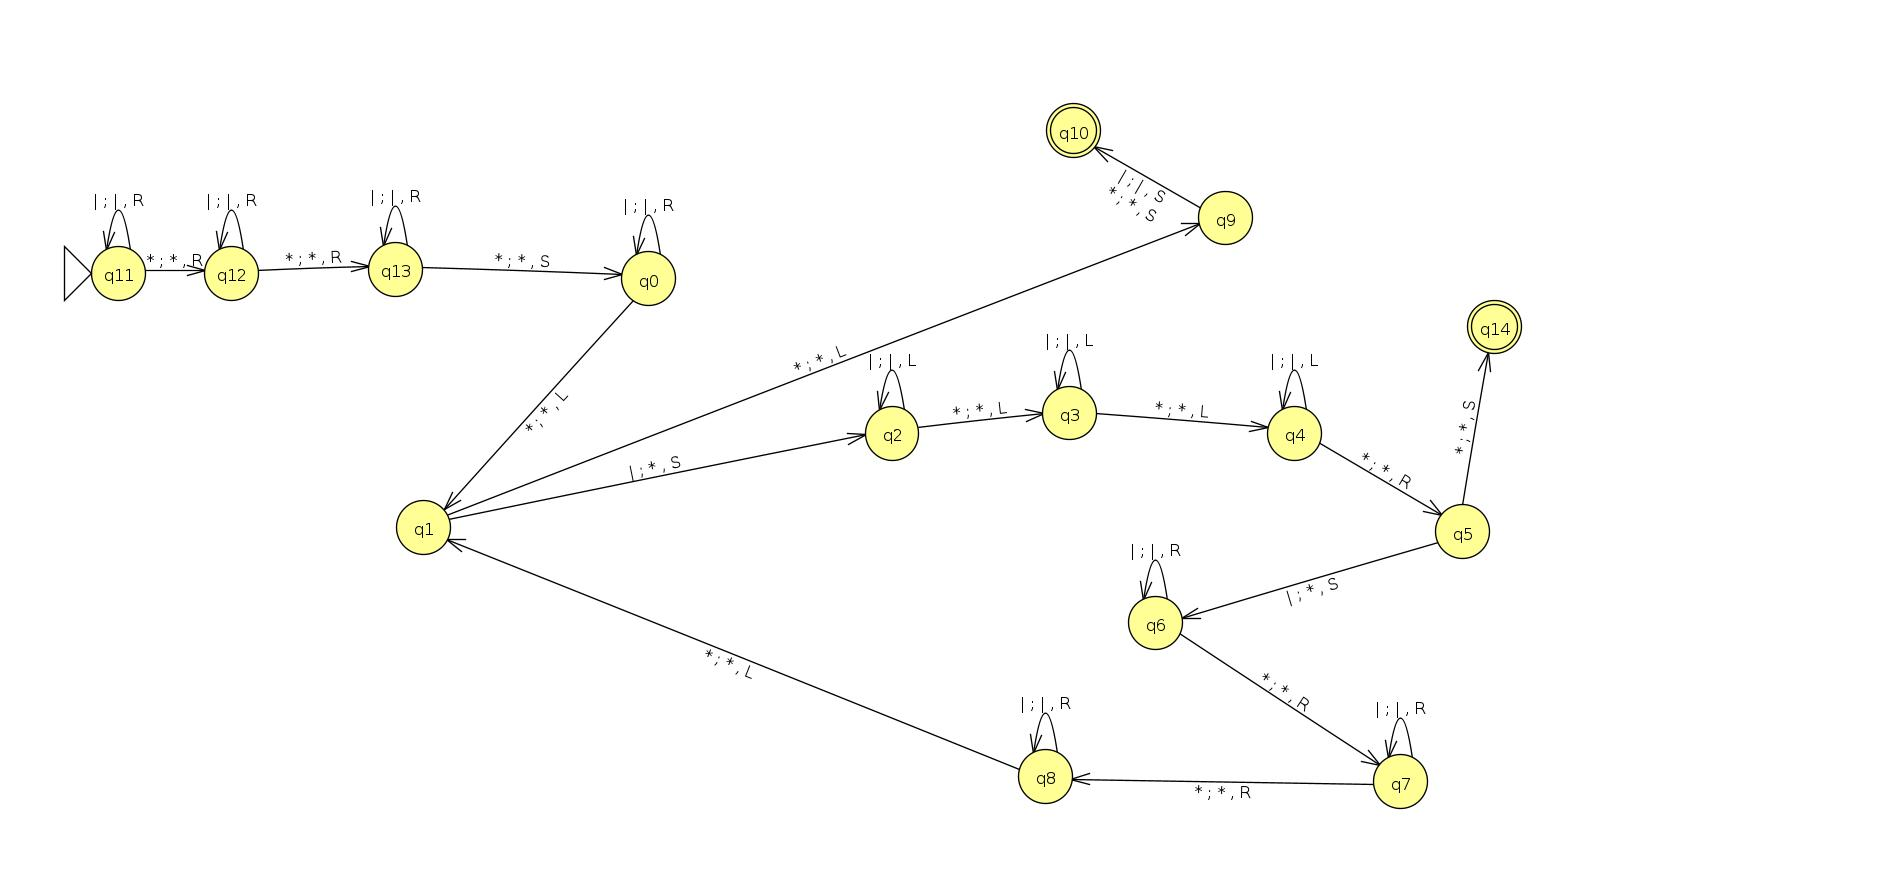
\includegraphics[width=20cm]{TM.jpg}
\end{center}
Por la forma de la que está definida este programa, la instrucción parar no significa parar la máquina de Turing, sino que donde apunta la maquina en la expresión de cinta no cambie. Para parar la máquina definitivamente tenemos los estados finales. Cuando la máquina llega a un estado final, para definitivamente. Otro apunte, debido al programa, el estado inicial es $q_{11}$.\\
Si la mágina para sobre un $|$, la expresión es verdadera, si para sobre un *, la expresión es falsa.

\section*{Ejercicio 2:}
Definir mediante una función recursiva la suma de 3 naturales:\\
Planteo la funcion por recursión primitiva:
\begin{center}
    $f(x,y,z)=\left\{ 
\begin{array}{lcc}
    x+y                          & \text{si} & z=0\\
    f(x,y, z-1)+1 & \text{if} & z>0 
\end{array}\right.$
\end{center}
Por tanto, como ya hemos visto en el tema, la suma de dos naturales se define resursivamente como: $\langle \pi^1_1 | \sigma(\pi^3_3) \rangle $, por tanto, para hacer la suma, tal y como hemos definido ya la recursión primitiva es:
\begin{center}
    $\langle\langle \pi^1_1 | \sigma(\pi^3_3) \rangle | \sigma(\pi^4_4) \rangle$
\end{center}
Si realizamos alguna prueba en Octave, vemos que funciona:
\begin{center}
    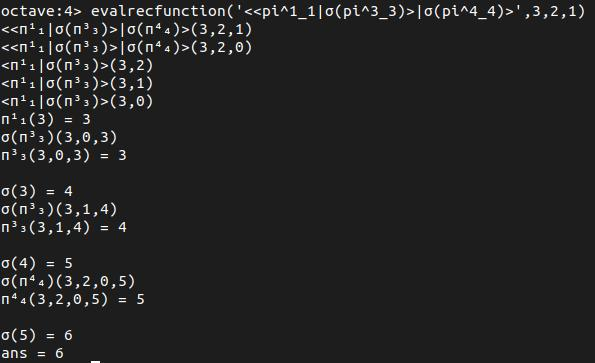
\includegraphics[width=10cm]{suma3.jpg}
\end{center}
\section*{Ejercicio 3:}
Realizar un programa WHILE que haga la suma de 3 naturales.\\
El razonamiento es facil, en una variable auxiliar iniciada a 0, se le va sumando mediante 3 while (1 para cada natural), unidad a unidad cada una de las variables, y al final el valor de esta variable auxiliar se le asigna a $X_1$ que es quien obtiene el resultado final del programa. 

\whileprogram{Q}{3}{
}{s}
\begin{whilecode}[H]

 \WhileSC{$X_1 \not = 0$}{

  $X_4 \Assig X_4 + 1$\;
  $X_1 \Assig X_1 - 1$\

 }
 \WhileSC{$X_2 \not = 0$}{

  $X_4 \Assig X_4 + 1$\;
  $X_2 \Assig X_2 - 1$\

 }
 \WhileSC{$X_3 \not = 0$}{

  $X_4 \Assig X_4 + 1$\;
  $X_3 \Assig X_3 - 1$\

 }
 $X_1 \Assig X_4$\

\end{whilecode}

\end{document}
